% !TeX spellcheck = en_US 
\chapter{Forensic audit and its computer support}


\komentar{na zacatek shrnout co vsechno obsahuje tato kapitola. asi tak takhle:}


This chapter strives to define and explain the meaning of the term "forensic audit" as well as other therms related to this field. We demonstrate typical roles and outline the process.
\komentar{az bude kapitola dopsana, zkontrolovat, zda toto odpovida} 

%\section{Matters of forensic audit}
%\komentar{nelibi se mi, pridat do jinych casti a zrusit}
%Forensic audit is a specialization within a field of accounting that examines and evaluates evidence concerning unproven statements for possible use as evidence in court. Forensic audit is usually used in case there is a suspicion in certain company there is a crime being committed. The background of the investigated case is rather diverse. A customer can be, for example, a CEO  who wants to examine the functioning of one of the sub-divisions of a controlling company. There can be a suspicion of some fraudulent activity or the need of forensic audit can be closely unspecified.

\section{Definition of forensic audit}
The term "forensic" can be defined in multiple ways. According to merriam-webster dictionary \komentar{citace http://www.merriam-webster.com/dictionary/forensic} the definition is "relating to the use of scientific knowledge or methods in solving crimes". The term "audit" is explained in the same dictionary as "a complete and careful examination of the financial records of a business or person". \komentar{citace http://www.merriam-webster.com/dictionary/audit}

The essence of forensic audit is to discover and investigate fraudulent intentions and fraudulent behavior. 

A common mistake in the definition of forensic audit is to confuse it with financial audit. The aim of financial audit is to verify whether financial statements are fairly stated in accordance with accounting standards. Financial auditors search for material errors or other misstatements in the accountancy.

On the other hand the ultimate goal of forensic audit is to examine existing or gained suspicion and procure evidence concerning possible fraudulent behavior. Deceptive scenarios are discovered in the process of forensic audit and evidence together with a documentation that is usable for subsequent course of action is gathered. As a matter of principle forensic auditors are not expected to express their opinion on the guilt or innocence of suspects.


%\section{When to use forensic audit}
%\komentar{asi spis nez priklady popsat za jakych situaci...}
%\sediva{\blindtext}

%=============================ze stare BP========================================
\section{Types of investigation}

The range of types of situation that forensic auditor can be asked to investigate is really wide. Basically any kind of suspicion on potentially bad behavior can be an impulse for investigation. However, not all kinds of crimes are of our interest. 


druhy zlocinu obecne
ktere z nich forenzni audit neresi
ktere z nich se jako pripady FA vyskytuji casteji
=>fraud

jine souvisejici oblasti forenzniho auditu
- specializace jako digital forensis etc.
vyuzitelne v ruznych pripadech na dilci vysetrovani
obnova dat - cesnet-man prednaska
(=> mohou se vyskytovat i dilci zakazky, kde se nezkouma komplexni situace ale napriklad jen obnovuji dulezita data, nebo analyzuji jednodussi pripady)


co nas zajima nejvice










The forensic auditor could be demanded to examine various sorts of fraud. To analyze the extensive area of examinations that could be completed, these sorts of fraud can be classified into three categories. The first category containing frauds such as conflict of interest, extortion or bribery. Approximately one third of fraudulent activities is somehow connected to corruption.In the second category we can find acts of cash theft, fraudulent disbursement or misuse of assets. This category can be generally called asset misappropriation and activities related to it are actually the most common frauds. All financial statement frauds may be considered as the third separate category, including all the deliberate misinterpretation of financial reporting standards or manipulation with obligations to improve analyses of liquidity. 



\subsection{Asset misappropriation}
Clearly the most widely recognized frauds are those including resource misappropriations and there are various sorts of misrepresentation which fall into this classification. The basic element is the burglary of money or different resources from the organization, for instance: 

\begin{itemize}
\item Cash burglary – the taking of physical money, for instance insignificant amount of money, from the premises of an organization.
\item Fraudulent payment – organization trusts being utilized to make fake installments. Regular illustrations incorporate charging plans where installments are made to an imaginary supplier and finance plans where installments are made to invented workers that are frequently known as 'apparition representatives'.
\item Inventory replicas – the robbery of stock from the organization. 
\item Misuse of benefits – representatives utilizing organization resources for their own interest.
\end{itemize}


\subsection{Financial statement fraud}

This is deceitful money related reporting, and is a kind of misrepresentation that causes a material misquote in the budgetary proclamations. It can incorporate planned distortion of bookkeeping records; exclusion of exchanges, equalizations or exposures from the budgetary explanations; or the misuse of money-related reporting guidelines. This is regularly done with the goal of giving the budgetary proclamations a specific inclination, for instance covering liabilities to enhance any examination of liquidity.
%============================^ze stare BP^=======================================





\section{How to prepare for a forensic audit}
%\komentar{v hrubych rysech jak to probiha (to co uz mam sem patri), na zaklade toho, co jsem zjistila, FA funguje takto:...\\}

On the basis of what we have found the process of forensic audit works as follows. When it is decided that certain situation will be investigated in forensic audit it is important to prevent all investigated individuals to access all related documents and electronic evidence. It is also recommended to limit their access to corporate information systems. 

Next step is to formulate properly the assignment. To define the extent and expectations on the outcome of forensic audit. To prevent a misunderstanding the assignment should be as specific and detailed as possible. It is best to choose the right audit company according to references and their experience with similar cases as the one we have specified.

When a client contacts an audit company with an assignment they usually schedule a meeting together, formulate sign and accept the assignment. The ordering party should be prepared to provide access to corresponding electronic and paper-like documentation as well as accept the fact that auditors are going to question employees and case-related person. On the other hand the audit company undertakes to refrain from sharing all the confidential information with third parties.A team of specialists that are convenient to the assignment is formed and the inspection is launched. 

The following steps of the precise method of forensic audit are not definite. The ability to adapt in new situations is one of many essential capabilities for the team of forensic auditors. The variety of investigated cases is so vast that there is no universally valid and precise course of action in the same time. Therefore on this place we present only general methodology of forensic audit. Several selected methods of forensic audit will be described later in this document. \komentar{link na spravne misto!}

\section{General methodology of forensic audit}
In this section we present basic phases that are used while performing forensic audit. This process is most commonly divided into four stages: Accumulation, Examination, Analysis and Reporting. This basic methodology starts after the  selection of the audit company and after the specification of the assignment; at the same time when the real work of forensic auditors begins.

\begin{figure}[h]
	\begin{center} 
	%\missingfigure{Obrazek demonstrujici forenzni audit.}
	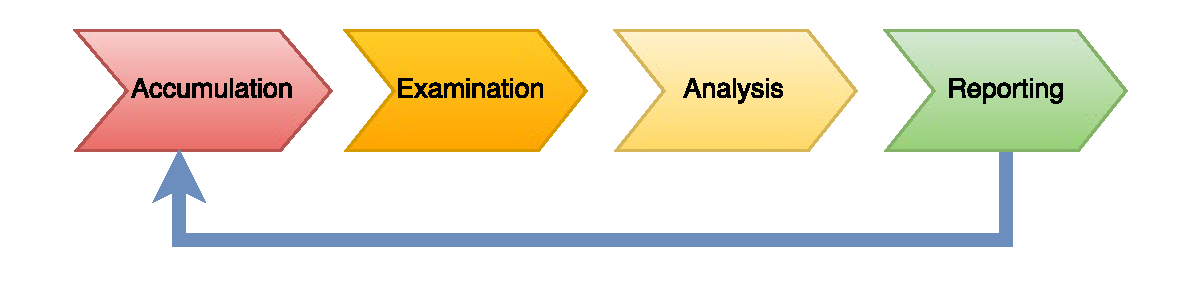
\includegraphics[width=1.0\textwidth]{img/general_methodology.pdf}
	\end{center}
	\caption{\komentar{General methodology of forensic audit}}
\end{figure}

%vvvvvvvvvvvvvvvvvvvvvvvvvvvvvvvvvvvvvvvvvvvvvvvvvvvvvvvvvvvvvv
\paragraph{Accumulation:} 
The main purpose of this stage is to acquire as much usable data as possible. It means recognize possible sources of data and provide backup record. All the sources of data and information, including necessary cross examination and other sources of evidence, should be utilized in this phase. All the information from the conceivable sources of pertinent information should be gained.

\paragraph{Examination:}
Examinations include forensically preparing all the gathered data. This can be done using a blend of computerized and manual systems to survey and concentrate specifically compelling information. 

\paragraph{Analysis:}
The following period of the procedure is to investigate the consequences of the examination, using legitimately reasonable routines and systems. The aim is to infer helpful data that addresses the inquiries that were the impulse for performing the accumulation and examination. \komentar{grrrrrr...}


\paragraph{Reporting:}
The last stage is reporting the consequences of the investigation, which may include depicting the activities utilized, clarifying how devices and methods were chosen, figuring out what different activities should be performed and giving proposals to change to approaches, rules, techniques, apparatuses, and different parts of the measurable procedure. 


%^^^^^^^^^^^^^^^^^^^^^^^^^^^^^^^^^^^^^^^^^^^^^^^^^^^^^^^^^^^^^^
%\sediva{\blindtext}





%===================================================================================
\section{Use case diagram of forensic audit in general}

As we see it there are three basic roles in forensic audit. A customer who wants a particular case to be investigated. The action of the customer is to assign the order to a audit company. A representative of the company i.e., for example, forensic auditor takes over the order and starts the investigation. The operations requiring specialized skills can be delegated to an expert from the proper field. Forensic auditors together with specialists then investigate the case and search for the evidence. In the end of the investigation the auditor reports the conclusion to the customer. 

\begin{figure}[h]
	\begin{center} 
	%\missingfigure{Velky obrazek vsech zainteresovanych stran - f.auditor, datovy analytik pro FA, zakaznik (zadavatel, materska spolecnost)}
	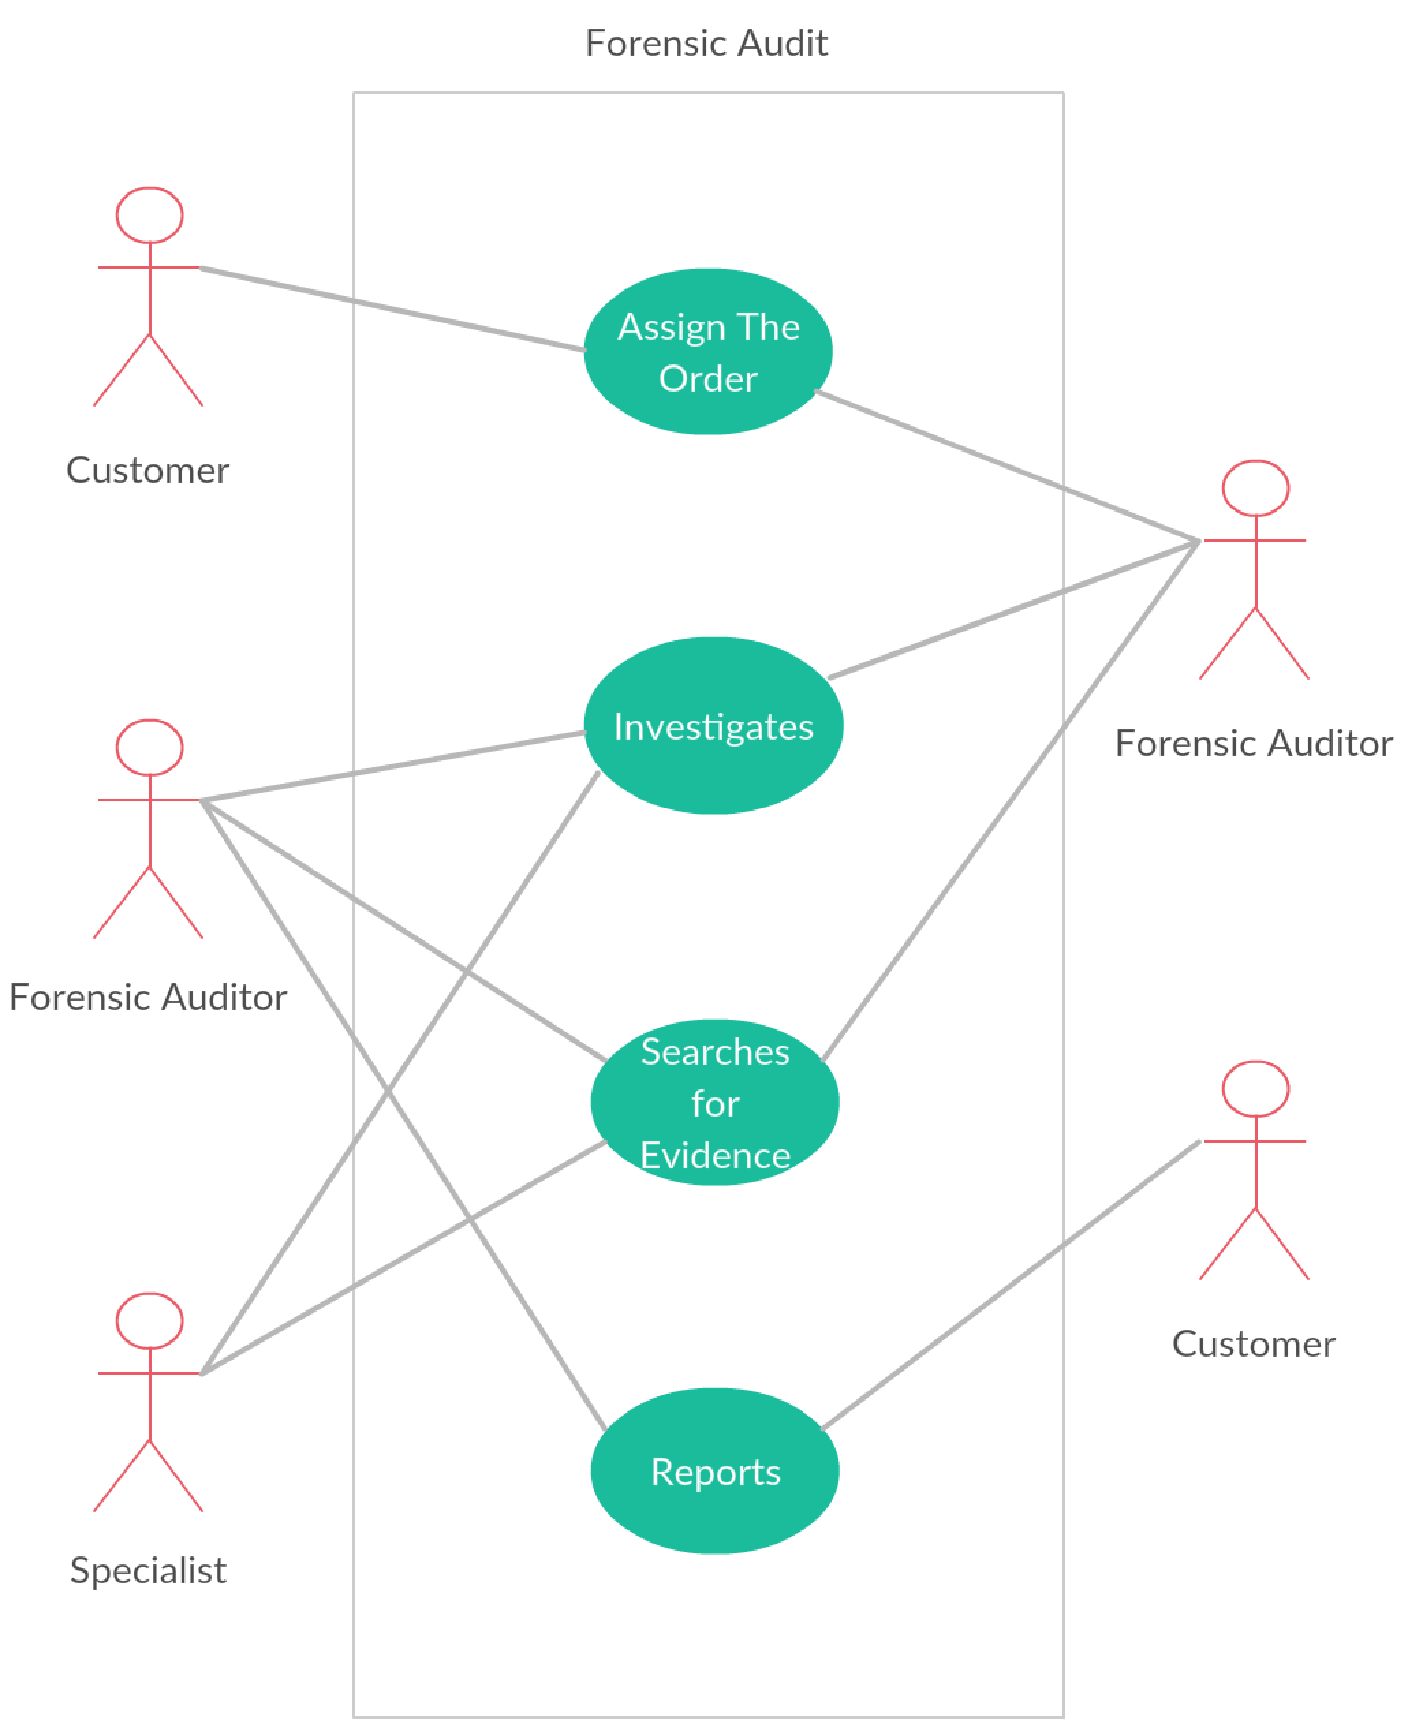
\includegraphics[width=0.8\textwidth]{img/usecase/use_case-FA_general2.pdf}
	\end{center}
	\caption{Use case diagram of forensic audit in general}
\end{figure}


\komentar{\section{co sem jeste zahrnout:}}
\komentar{
	VIZE: Rozdelit obecne druhy odhalovaneho chovani. Zahrnout vseobecne veskerou tresnout cinnost - nejspis podle zakona? Z techto oblasti vyelimimovat vsechny, pro ktere nema cenu uvazovat pocitacovou podporu (nasilne ciny, prepadeni, kradeze hmotneho majetku, pravni dokumenty? atd.). \\ Zbyle tak nejak rozdelit do skupin podle toho, jaky druh pocitacove podpory je obecne vyuzitelny. Pak se mozna pokusit k sobe priradit dany precin a metodu. Z metod nechci zminovat konkretni SW, ale spise obecne oblasti reseni - jak vyuzivame data mining, fuzzy logiku, strojove uceni (nebo alespon co to je a ze se take muze vyuzit), kvantitativne analyticky SW, forenzni toolkity na obnovu dat a podobne.
}

\komentar{
Priklady

·         Pan X, reditel ceske pobocky mezinarodni firmy\\

o   ma bratra, ktery mu dodava papir 500 Kc za balik.\\

·         Pani Y, ucetni spolecnosti\\

o   zauctuje falesnou fakturu na zalevani kvetin ve vysi 20 000 Kc (s vedomim pana Novaka)\\

·         Pan Z, spravce budovy\\

o    zamestna na parkovou upravu pred spolecnosti firmu, ktera mu stavi rodinny dum\\

Typy problemu\\

·         Predrazene dodavky\\

·         Fiktivni faktury\\

·         Nesoulad podnikani dodavatele a faktury\\

·         Paralelni spoluprace\\
}
%\dotaz{Z predchozi vize chci prejit v dalsi kapitole zpet k obecne metodologii a diagramu z ARISu. Nevim, jak na to plynule navazat aby to davalo celkove hlavu a patu. Snad me jeste neco napadne.}




